\documentclass[9pt]{beamer}
\usetheme[progressbar=head,numbering=fraction]{metropolis}
\usepackage[utf8]{inputenc}
\usepackage[T1]{fontenc}
\usepackage{lmodern}

\usepackage{empheq}
\makeatletter
\colorlet{shadecolour}{blue!30}
\newcommand\Ashaded[1]{\let\bgroup{\romannumeral-`}\@Ashaded#1&&\ENDDNE}
\def\@Ashaded#1&#2&#3\ENDDNE{%
\ifnum0=`{}\fi \setbox \z@
\hbox{$\displaystyle#1{}\m@th$\kern\fboxsep \kern\fboxrule }%
\edef\@tempa {\kern \wd\z@ &\kern -\the\wd\z@ \fboxsep
\the\fboxsep }\@tempa \colorbox{shadecolour}{$#1#2 $}%
}
\colorlet{bgcolour}{yellow!20}
\colorlet{rulecolour}{blue!30}
\newcommand\Acolorboxed[1]{\let\bgroup{\romannumeral-`}\@Acolorboxed#1&&\ENDDNE}
\def\@Acolorboxed#1&#2&#3\ENDDNE{%
  \ifnum0=`{}\fi \setbox \z@
    \hbox{$\displaystyle#1{}\m@th$\kern\fboxsep \kern\fboxrule }%
    \edef\@tempa {\kern \wd\z@ &\kern -\the\wd\z@ \fboxsep
        \the\fboxsep\fboxrule \the\fboxrule }\@tempa \fcolorbox{rulecolour}{bgcolour}{$ #1#2 $}%
}
\makeatother

\usepackage{amsfonts,amsmath}
\allowdisplaybreaks


%% X color
\definecolor{darkblueX}{RGB}{0,62,92}
\definecolor{lightblueX}{RGB}{0,104,128}
\definecolor{verylightblueX}{RGB}{212,232,239}
\definecolor{redX}{RGB}{169,32,33}




%% Font

\setbeamerfont{framesubtitle}{size=\tiny}
\setbeamerfont{alerted text}{shape=\bfseries}




%\usepackage[export]{adjustbox}

% Tighter itemize
\expandafter\def\expandafter\normalsize\expandafter{%
    \normalsize%
    \setlength\abovedisplayskip{1pt}%
    \setlength\belowdisplayskip{1pt}%
    \setlength\abovedisplayshortskip{1pt}%
    \setlength\belowdisplayshortskip{1pt}%
}

\expandafter\def\expandafter\small\expandafter{%
    \small%
    \setlength\abovedisplayskip{1pt}%
    \setlength\belowdisplayskip{1pt}%
    \setlength\abovedisplayshortskip{1pt}%
    \setlength\belowdisplayshortskip{1pt}%
}

%\usepackage{beamerX}
\newcommand{\alertmath}[1]{\textcolor{blue}{\boldsymbol{#1}}}
%\setboolean{displaylogo}{false}

\AtBeginSection[]
{
\begin{frame}
        \frametitle{Outline}
        \tableofcontents[currentsection]
   \end{frame}
}
\AtBeginSubsection[]
{
\begin{frame}
        \frametitle{Outline}
        \tableofcontents[currentsection,currentsubsection]
   \end{frame}
}

\setbeamertemplate{frametitle continuation}[from second][]

\usepackage{graphicx}%

\newcommand{\parinc}[2]{\parbox[c]{#1}{\includegraphics[width=#1]{#2}}}
\newcommand{\parinch}[3]{\parbox[c][#2]{#1}{\includegraphics[width=#1]{#3}}}
\newcommand{\parincb}[3]{\parbox[c]{#1}{\includegraphics[width=#1,height=#2]{#3}}}

\usepackage{color}
\newcommand{\red}[1]{\textcolor{red}{#1}}

\usepackage{tikz}


\usepackage{scalerel,stackengine}
\stackMath
\newcommand\reallywidehat[1]{%
\savestack{\tmpbox}{\stretchto{%
  \scaleto{%
    \scalerel*[\widthof{\ensuremath{#1}}]{\kern-.6pt\bigwedge\kern-.6pt}%
    {\rule[-\textheight/2]{1ex}{\textheight}}%WIDTH-LIMITED BIG WEDGE
  }{\textheight}% 
}{0.5ex}}%
\stackon[1pt]{#1}{\tmpbox}%
}

\newcommand{\grad}{\nabla}
\newcommand{\ind}[1]{\mathbf{1}_{#1}}

\DeclareMathOperator{\limSup}{limsup}%
\DeclareMathOperator{\limInf}{liminf}%
\DeclareMathOperator*{\argmax}{argmax}%
\DeclareMathOperator*{\argmin}{argmin}%
\DeclareMathOperator*{\supp}{Supp}%
\DeclareMathOperator{\pen}{pen}
\DeclareMathOperator{\dom}{dom}
\DeclareMathOperator{\price}{price}
\DeclareMathOperator{\sign}{sign}
\DeclareMathOperator{\KL}{KL}
\DeclareMathOperator{\Proj}{Proj}
\DeclareMathOperator{\Span}{span}


\DeclareMathOperator*{\tr}{tr}
\DeclareMathOperator*{\ra}{rank}
\DeclareMathOperator*{\conv}{conv}
\DeclareMathOperator{\ve}{vec}
\DeclareMathOperator{\diag}{diag}



\newcommand{\Espe}{\mathbb{E}}
\newcommand{\Vari}{\mathbb{V}}
\newcommand{\Cova}{\mathbb{C}\text{ov}}
\newcommand{\Prob}[2][]{\mathds{P}_{#1}\left\{#2\right\}}
\newcommand{\Esp}[2][]{\Espe_{#1}\left[#2\right]}
\newcommand{\Var}[2][]{\Vari_{#1}\left[#2\right]}
\newcommand{\Cov}[2][]{\Cova_{#1}\left[#2\right]}
\newcommand{\ud}{\textup{d}}
\newcommand{\charac}{\mathbf{1}}

\newcommand{\vecX}{\textbf{X}}
\newcommand{\vecx}{\textbf{x}}
\newcommand{\transp}[1]{{#1}^t}

\usepackage{pdfpages}
\usepackage{tikz}
\usepackage{dsfont}
\usepackage{ragged2e}
\usepackage{mathabx}
\usepackage[style=alphabetic, citestyle = authoryear, maxcitenames=2,backend=biber]{biblatex}
\addbibresource{../deeplearning_course.bib}
%Compile pdflatex, biber, pdflatex, pdflatex

\usepackage{graphicx}
\graphicspath{{}}
\usepackage{ragged2e}

\newcommand\citem[1]{{\scriptsize[\citetitle{#1}, \cite{#1}]}}
\DeclareMathOperator{\prox}{prox}
\newcommand{\eps}{\varepsilon}
\newcommand{\norm}[1]{\|#1\|}
\newcommand{\inr}[1]{\langle #1 \rangle}
\newcommand\redd[1]{\textcolor{red}{#1}}
\newcommand\blue[1]{\textcolor{blue}{#1}}
\newcommand\iid{\textit{i.i.d.}}
\newcommand\bW{\textbf{W}}
\newcommand\R{\mathds{R}}
\newcommand\bx{\mathbf{x}}
\renewcommand\pen{\textrm{pen}}
\newcommand{\E}{\mathds{E}}
\newcommand{\V}{\mathds{V}}
\newcommand{\cov}{\mathds{C}}
\renewcommand{\P}{\mathds{P}}

\usepackage{ifthen}
\newboolean{correction_bool}
\setboolean{correction_bool}{false}
\newcommand{\ifinclude}[1]{\ifthenelse{\boolean{correction_bool}}{#1}{}}


\title{Introduction to neural networks}

\author{}
\date{}

\begin{document}

\author[S. Le Corff]{\textcolor{violet}{Models and back propagation}\\ {\em {\small \textcolor{violet}{}}}}

\begin{frame}
  \titlepage
\end{frame}


 \section{Motivation in Machine Learning}


\begin{frame}
	\frametitle{General optimization problem}
	
\alert{Parameter inference in machine learning} often boils down to solving

\begin{equation*}
\argmin_{w \in \R^d} \ell_n(w) + g(w)\,,
\end{equation*}

with $\ell_n$ a \alert{goodness-of-fit functio  based on a loss $\ell$},

\begin{equation*}
\ell_n(w) = \frac 1n \sum_{i=1}^n \ell(w,y_i,  x_i \rangle)
\end{equation*}

 and

\begin{equation*}
g(w) = \lambda \pen(w)\,,
\end{equation*}

where $\lambda>0$ and \alert{$\pen(\cdot)$ is some penalization function}.

%Examples of penalization functions:

$\rightharpoondown$ \textcolor{violet}{$\pen(w) =  \|w\|_2^2$ (Ridge).}

$\rightharpoondown$ \textcolor{violet}{$\pen(w) = \|w\|_1$ (Lasso)}.


\end{frame}


\begin{frame}
	\frametitle{General optimization problem - Regression}
	
In a regression setting, for all $1\leqslant i \leqslant n$, 
$$
Y_i = f_\star(X_i) + \varepsilon_i\,,
$$
where the $(\varepsilon_i)_{1\leqslant i\leqslant n}$ are i.i.d. centered random variables in $\mathbb{R}^M$, $X_i\in\mathbb{R}^d$ and \alert{$f_{\star}$ is an unknown function}.  

\vspace{.2cm}

The standard approach to estimate the parameters is by \alert{minimizing the mean square error}:
$$
\ell_n:\theta \mapsto  \frac{1}{n} \sum_{i=1}^n\left\|f_{\theta}(X_i) - Y_i\right\|^2\,,
$$
where \alert{$f_{\theta}$ is a nonlinear parametric function} used to estimate the unknown function $f_\star$.

\end{frame}

\begin{frame}{Gradient descent algorithm}
	


\textbf{\textcolor{violet}{Gradient descent}}
		
\alert{Input}: Function $\ell_n$ to minimize, initial vector $\theta^{(0)}$, $k=0$.

\medskip 
	
	
\alert{Parameters}: step size $\eta>0$.

\medskip
	
While \textit{not converge} do


\hspace{2cm} $\rightharpoondown$ $\theta^{(k+1)} = \theta^{(k)} - \eta_{k+1} \nabla \ell_n(\theta^{(k)})$.

\hspace{2cm} $\rightharpoondown$ $k = k+1$.

\medskip

\alert{Output}: $\theta^{(n_*)}$ where $n_*$ is the last iteration.

	
\end{frame}



\section{Neural networks}

\begin{frame}{A neuron}

\begin{center}
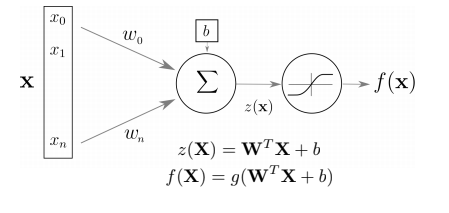
\includegraphics[width = 0.75\textwidth]{neuron.png}
\end{center}

$\rightharpoondown$ $X$ \alert{input in $\R^d$}.

$\rightharpoondown$ $z(X)$ \alert{pre-activation in $\R^M$}, with \alert{weight $W\in\R^{dxM}$} and \alert{bias $b\in\R^M$}.

$\rightharpoondown$ $g$ \alert{softmax function}.

\vspace{.3cm}

{\bf\textcolor{violet}{One neuron is a multi-class extension of the logistic regression model}}. 

\end{frame}

\begin{frame}{Layer of neurons and hidden states}

\begin{center}
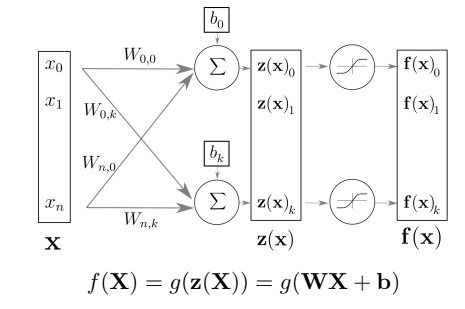
\includegraphics[width = 0.75\textwidth]{neuronlayer.png}
\end{center}

$\rightharpoondown$ $X$ \alert{input in $\R^d$}.

$\rightharpoondown$ $z(X)$ \alert{pre-activation in $\R^k$}, with \alert{weight $W\in\R^{dxk}$} and \alert{bias $b\in\R^k$}.

$\rightharpoondown$ $g$ \alert{any activation function} (nonlinear \& nondecreasing function).

$\rightharpoondown$ $f(X)$ \alert{hidden state} in $\R^k$ which may be used as input of a new neuron...


\end{frame}

\begin{frame}{Feed Forward Network}

\begin{center}
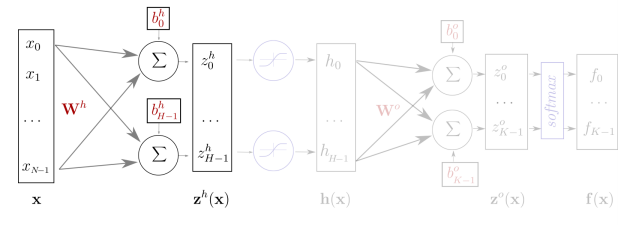
\includegraphics[width = 0.9\textwidth]{ffnn1.png}
\end{center}

$\rightharpoondown$ $X$ \alert{input in $\R^d$}.

$\rightharpoondown$ $z^h(X)$ \alert{pre-activation in $\R^H$}, with \alert{weight $W^h\in\R^{dxH}$} and \alert{bias $b^h\in\R^H$}.


\end{frame}

\begin{frame}{Feed Forward Network}

\begin{center}
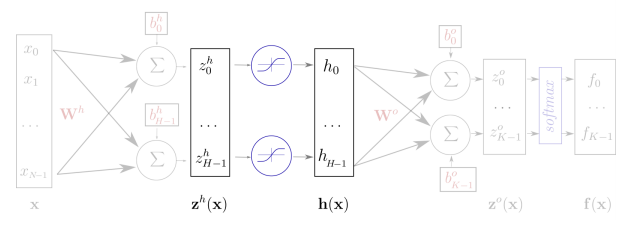
\includegraphics[width = 0.75\textwidth]{ffnn2.png}
\end{center}

$\rightharpoondown$ $X$ \alert{input in $\R^d$}.

$\rightharpoondown$ $z^h(X)$ \alert{pre-activation in $\R^H$}, with \alert{weight $W^h\in\R^{dxH}$} and \alert{bias $b^h\in\R^H$}.

$\rightharpoondown$ $g$ \alert{any activation function} to produce $h\in\R^H$.
\end{frame}

\begin{frame}{Feed Forward Network}

\begin{center}
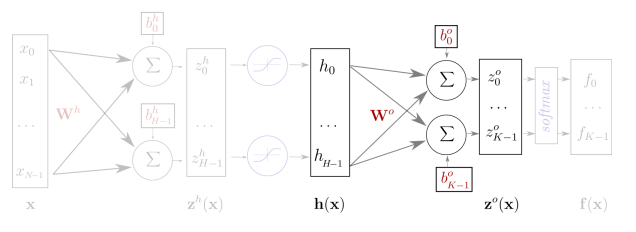
\includegraphics[width = 0.75\textwidth]{ffnn3.png}
\end{center}

$\rightharpoondown$ $X$ \alert{input in $\R^d$}.

$\rightharpoondown$ $z^h(X)$ \alert{pre-activation in $\R^H$}, with \alert{weight $W^h\in\R^{dxH}$} and \alert{bias $b^h\in\R^H$}.

$\rightharpoondown$ $g$ \alert{any activation function} to produce $h\in\R^H$.

$\rightharpoondown$ $z^o(X)$ \alert{pre-activation in $\R^M$}, with \alert{weight $W^o\in\R^{HxM}$} and \alert{bias $b^o\in\R^M$}.

\end{frame}

\begin{frame}{Feed Forward Network}

\begin{center}
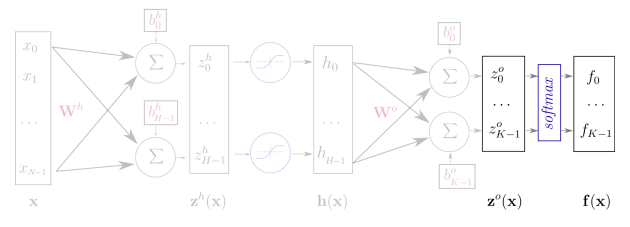
\includegraphics[width = 0.75\textwidth]{ffnn4.png}
\end{center}

$\rightharpoondown$ $X$ \alert{input in $\R^d$}.

$\rightharpoondown$ $z^h(X)$ \alert{pre-activation in $\R^H$}, with \alert{weight $W^h\in\R^{dxH}$} and \alert{bias $b^h\in\R^H$}.

$\rightharpoondown$ $g$ \alert{any activation function} to produce $h\in\R^H$.

$\rightharpoondown$ $z^o(X)$ \alert{pre-activation in $\R^M$}, with \alert{weight $W^o\in\R^{HxM}$} and \alert{bias $b^o\in\R^M$}.

$\rightharpoondown$  Apply the \alert{softmax function to produce the output}, i.e. $\mathbb{P}(Y=m|X)$ for $1\leqslant m \leqslant M$.
\end{frame}

\begin{frame}{Activation functions}

\begin{center}
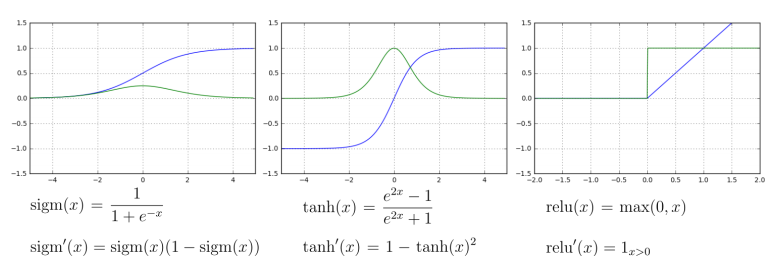
\includegraphics[width = 0.9\textwidth]{activations.png}
\end{center}

$\rightharpoondown$ As there is no modelling assumptions anymore, \alert{virtually any activation function} may be used. 

$\rightharpoondown$ The rectified linear unit (RELU) activation function $\sigma(x) = \mathrm{max}(0,x)$ and its extensions are the default recommendation in modern implementations  (Jarrettet al., 2009; Nair and Hinton, 2010; Glorot et al., 2011a), (Maas et al.,2013),  (He et al., 2015). One of the major motivations arise from the \alert{gradient based parameter optimization which is numerically more stable with this choice}. 

\end{frame}


\section{Backpropagation}

\end{document}


